% UFO camera developers manual
%

\chapter{Developers manual}

\section{Hardware}

\subsection{High-throughput architecture}

The CMOS-image sensor receives a request for the new frame in combination with the defined exposure time. When the integration time is finished, the image stored in the pixelmatrix (global shutter) is read out sequentially, row-by-row. The pixel values are then passed to a column ADC cell, which ADC conversion is performed. Then, in 10bit/pixel configuration, the digital signals are read out over 16 parallels LVDS (low voltage differential signal) channels where each LVDS channel reads out 128 adjacent columns of the array. Control registers are used for the programming of the sensor. Overview is displayed in Figure \ref{fpga-arch}.

\begin{figure}
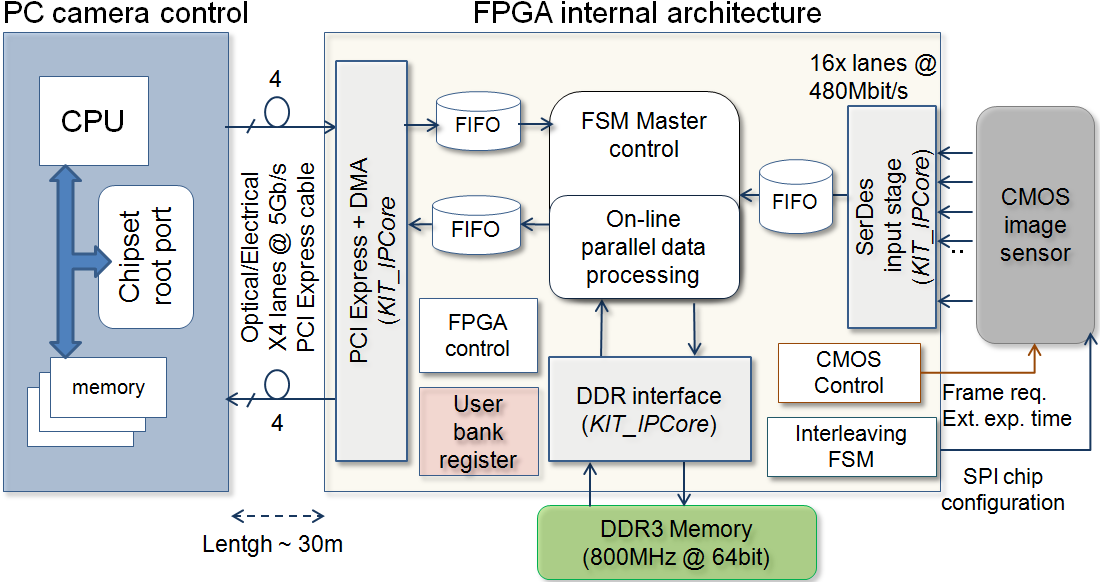
\includegraphics[width=\textwidth]{images/Figure_3_5.png}
\caption{\label{fpga-arch} Readout chain and FPGA architecture.}
\end{figure}


In order to read out the CMOS sensor as fast as possible, a PCI Express interface is used to transfer the data arriving from the mother board directly to the computer embedded memory. A PCI Express x4 lane generation 2 standard, with a theoretical bandwidth of 20 Gbit/s, is used. The achieved bandwidth is only limited by the speed grade of the FPGA. Direct Memory Access (DMA) is used to transfer the data from the camera to the central system memory and vice versa.

Addressable 32-bit user bank registers are implemented in the dedicated Base Address Registers (BAR) space. Bank registers are used to write/read the status/configurations of the DMA engines, the CMOSIS chip and the FPGA logic. Unused address locations of the bank can be used by further user applications. More information about the bank registers is given in chapter[[?]. The DDR (Double Data Rate) memory device is used for both temporary frame data storage before the transferring of the data and for an on-line data elaboration.

Camera has full access of the pixel parameters in order to adapt the pixel response at any experiment condition, like adjustable image exposure time and pixel dynamic range, noise threshold, mask, analog gain, etc. Continuous data acquisition at full speed for each frame rate condition without any readout dead time is also achieved. This camera can easily be extended to any available CMOS-image sensor.


\subsection{Image sensor CMOSIS CMV2000}

The CMV2000 is a high speed CMOS image sensor with 2048 by 1088 pixels (2/3 optical inch) developed for machine vision applications. The image array consists of 5.5$\mu$m x 5.5$\mu$m pipelined global shutter pixels which allow exposure during read out, while performing CDS operation. The image sensor has sixteen 10- or 12-bit digital LVDS outputs (serial). The image sensor also integrates a programmable gain amplifier and pixel threshold. Each channel runs at 480 Mbps maximum. Higher frame rates can be achieved in row-windowing mode or row-subsampling mode. These modes are all programmable using the SPI interface. All internal exposure and read out timings are generated by a programmable on-board sequencer. External triggering and exposure programming is a sensor feature which is also implemented in the camera. Extended optical dynamic range can be achieved by using piecewise feature of the sensor.

Sensor features and characteristics:
\begin{itemize}
\item  2048 * 1088 active pixels on a 5.5$\mu$m pitch
\item Frame rate 270 frames/sec @10bit and 70 frames/s @12bit
\item row windowing capability
\item X-Y mirroring function
\item Master clocks: 5-48MHz and 50-480MHz (LVDS)
\item 16 LVDS-outputs @480MHz multiplexable to 4 at reduced frame rate
\item LVDS control line with frame and line information
\item LVDS DDR output clock to sample data on the receiving end
\item 10 bit ADC output at maximum frame rate, 12 bit ADC at reduced frame rate
\item Multiple High Dynamic Range modes supported
\item On chip temperature sensor
\item On chip timing generation
\item SPI-control
\item 3.3V signaling
\item Full well charge: 13.5Ke-
\item Dark noise: 13e- RMS
\item Dynamic range: 60 dB
\item Extended dynamic range: Piecewise linear response or interleaved read-out • Dark current: 125 e/s (@ 25C die temp) (from datasheet of the sensor)
\item Maximum power consumption: 600mW (from datasheet of the sensor)
\end{itemize}

Please look at the CMV2000 datasheet for more information regarding the sensor, and additional CMOSIS white papers regarding recommended register settings \cite{CMOSIS:CMV2000}. Also, in section \ref{camera_char} is given the overview of the sensor characterization for several different parameters.



\subsection{Data format}

The UFO camera uses a special data format to be able to send images and trigger 
information in a compact form. The format needs also to ensure data integrity. 
In case of transmission errors the information can partly be recovered. 

The data is send frame by frame.
Each frame consist of the HEADER, DATA PAYLOAD and TAIL.


\subsubsection{Header}

HEADER contains 8 word of information:

\begin{verbatim}
DHEADER_1 DHEADER_2 DHEADER_3 DHEADER_4
DHEADER_5 DHEADER_6 DHEADER_7 DHEADER_8

\end{verbatim}
Each DHEADER word has 32 bits.
\begin{verbatim}
DHEADER_1 = {4'h5, 28'h1111111};
DHEADER_2 = {4'h5, 28'h2222222};
DHEADER_3 = {4'h5, 28'h3333333};
DHEADER_4 = {4'h5, 28'h4444444};
DHEADER_5 = {4'h5, 28'h5555555};
DHEADER_6 = {4'h5, CMOSIS_start_addr[9:0], skip_lines[6:0], number_of_lines};
DHEADER_7 = {4'h5, 4'h5, frame_number};
DHEADER_8 = {4'h5, ADC_Resolution, Output_mode, FR_timestap};
\end{verbatim}

The values for \verb/ADC_resolution/ are given in the following table.

\begin{tabular}{|c|c|}
\hline
ADC resolution				& Value 	\\	
\hline
10-bit				& 0 \\
\hline
11-bit				& 1 \\
\hline
12-bit				& 2 \\
\hline
\end{tabular}

The parameter \verb/Output_resolution/ is given in the following table

\begin{tabular}{|c|c|}
\hline
ADC resolution			& Value 	\\	
\hline
16 outputs				& 0 \\
\hline
8 outputs-not used		& 1 \\
\hline
4 outputs				& 2 \\
\hline
2 outputs-not used		& 3 \\

\hline
\end{tabular}


\subsubsection{Tail}

The TAIL contains again 8 words.

\begin{verbatim}
TAIL_1 TAIL_2 TAIL_3 TAIL_4
TAIL_5 TAIL_6 TAIL_7 TAIL_8
\end{verbatim}

All TAIL fields are 32 bits wide. In total the tail has a length of 256 bits.
\begin{verbatim}
TAIL_1 = {4'h0, 28'hAAAAAAA};
TAIL_2 = {Status1};
TAIL_3 = {Status2};
TAIL_4 = {Status3};
TAIL_5 = {4'h0, 2'h0, app_addr_rd};
TAIL_6 = {4'h0, 2'h0, app_addr_wr};
TAIL_7 = {4'h0, 28'h0000000};
TAIL_8 = {4'h0, 28'h1111111};
\end{verbatim}


\subsubsection{Data}

Data payload is organized in blocks of 256 bits. One block contains the information of 16 pixel. Each block starts with a 32bit wide data block header. Depending on the mode of operation 16 x 10, 16 x 11 or 16 x 12bit of data are contained in the block. The rest of the data block is filled with zeros. At maximum ADC data with up to 14bit per pixel can be coded by this scheme.  

For 10bit data per pixel:
\[
\underbrace{Header}_{32bit} \; \; \underbrace{00000000}_{32bit} \;  \;\underbrace{00000000 }_{32bit} \; \; \underbrace{Pix\;ch0 \;  \; \ldots  \;  \;Pix\;ch15}_{160 \; bits}
\]

For the 12bit data per pixel:
\[
\underbrace{Header}_{32bit} \; \; \underbrace{00000000}_{32bit} \;  \; \underbrace{Pix\;ch0 \;  \; \ldots  \;  \;Pix\;ch15}_{192 \; bits}
\]


The data block header gives information on the position of the pixel in the images. 
The whole image is organized in 16 columns, each served by one channel.
One data block contains always the data of one pixel from each channel.
All the pixel in the block have the same relative position in the 16 columns. 
The position is given by row and column (called pixel number). 
The resulting pixel map is is shown below.

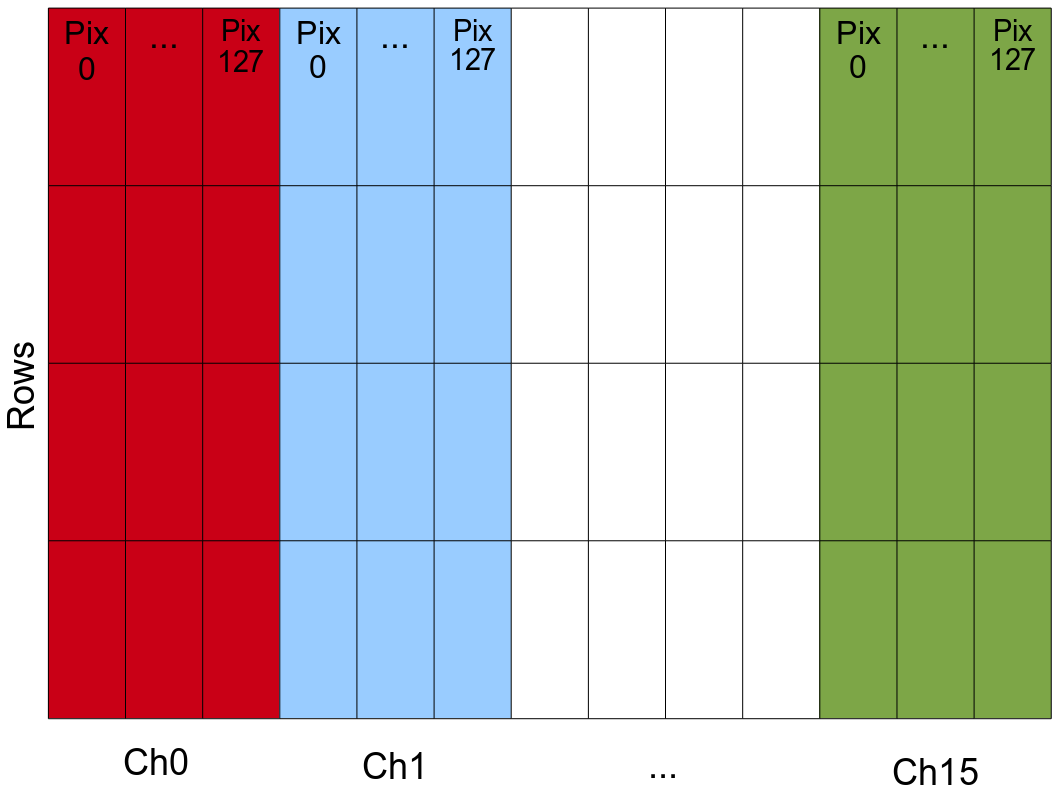
\includegraphics[width=0.8\textwidth]{images/pixel_map.png}

The format of the data block header is:
\begin{verbatim}
Header = {8'b10000000, pixel_size (4 bits), 
          1'b0, row_number (11 bits), 1'b0, pixel_number(7 bits)};
\end{verbatim}

In order to cover all pixel of the CMOSIS sensor CMV2000 the parameter \verb/pixel_number/ has values from 0 to 127 and \verb/row_number/ has value from 0 to 1088.

Example of a single data payload block with 10bit ADC values:
\begin{verbatim}
0x80a00000 0x00000000 0x00000000 0x595794d9  
0xd96c5257 0x6d5655e5 0x97059571 0xf5a96b59
\end{verbatim}




\section{Software}

The camera software splits in three parts. Interface to the camera hardware, a general camera interface library and specific decoding modules for the supported image sensors.

\subsection{Camera driver and tools -- pcitool}

The architecture of the software layer is presented in Figure 1.3. It includes a kernel module, an PCILIB library, command-line utility and a GUI.

\begin{figure}
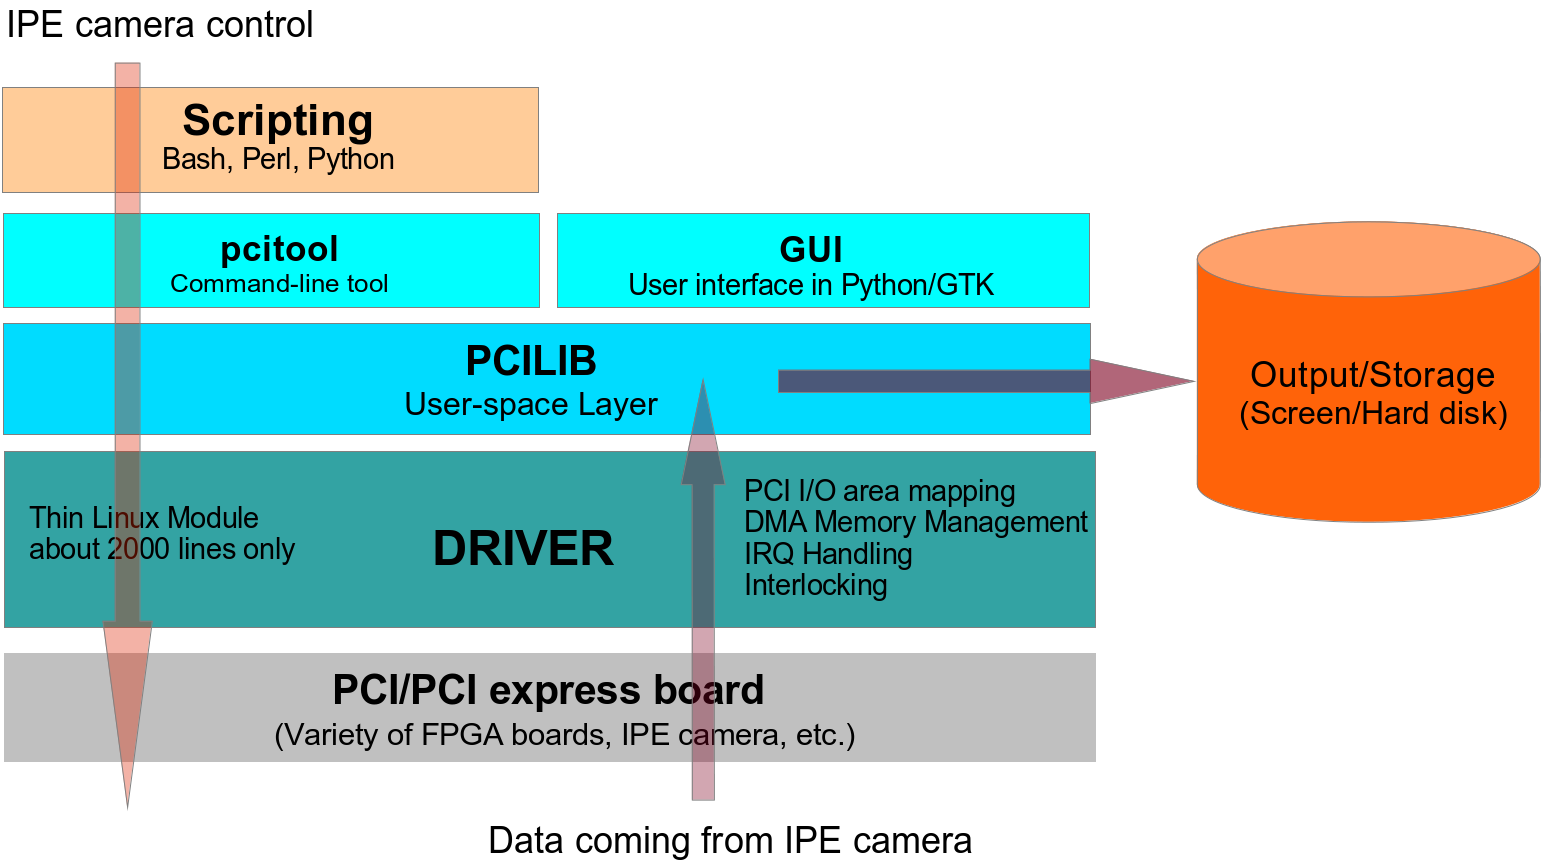
\includegraphics[width=\textwidth]{images/software_layer3.png}
\caption{\label{pcitool-arch} Software layer and data flow.}
\end{figure}

The kernel module is kept as small as possible. It is only responsible for de- vice configuration, interrupt counting, management of DMA buffers, and mapping of both PCI I/O space and DMA buffers into the userspace. All other functions in- cluding the actual implementation of DMA engine are realized in user space. Finally, the design of the driver allows fine grained scripting. For example, it is possible to start the DMA engine, set some registers to initiate DMA transfer, read data from DMA engine, make an attempt to process it, and if the wrong data is returned, analyze the status registers to find the signature of the error.

Scripts (using the pcitool) are used for the camera initialization, camera control, and for the main data acquisition. GUI can be used for data visualization in real time. GUI can also be used for data acquisition, but in such case, the maximum
frame rate is no more than 20 frames/s.



